\section{Primal Duel}

\frame{

\begin{figure}
\centering
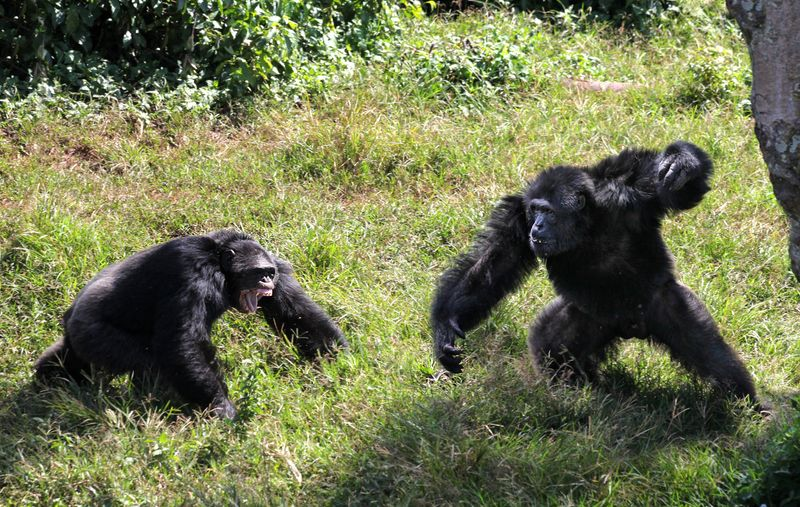
\includegraphics[width=0.8\textwidth]{slides/primal_duel/two_apes.jpg}
\end{figure}

}

\frame{

\frametitle{\secname}

\begin{itemize}
\item Optimization problems
\begin{itemize}
\item Find minimum/maximum of objective function
\item Variables must satisfy constraints
\end{itemize}
\pause
\item Initial formulation called the ``primal"
\pause
\item There is a transformation that moves primal constraints into objective function terms, and moves primal objective function terms into constraints
\begin{itemize}
\item The resulting formulation is called the ``dual"
\end{itemize}
\pause
\item Some optimization algorithms switch between primal and dual formulations
\begin{itemize}
\item \emph{Primal-dual} methods
\end{itemize}
% \item Depending on the type of optimization problem, either the primal and dual optimum are the same, or there exists a gap
% \begin{itemize}
% \item Strong vs weak duality
% \end{itemize}
% \pause
% \item 
\includegraphics[height=\baselineskip]{slides/primal_duel/simplex.png}

\end{itemize}

}
